\documentclass[twoside]{article}

\usepackage[a4paper, total={674pt, 426pt}, landscape]{geometry}
\usepackage{multicol}

\newcommand{\todo}[1]{\textcolor{red}{\textbf{TODO:} #1}}
\newcommand{\dyade}[1]{\overleftrightarrow{#1}}
\newenvironment{definition}[1]{\begin{tcolorbox}[title=Def.: #1, colback=white!,colframe=green!50!black]}{\end{tcolorbox}}

\titlespacing*{\section}{0pt}{.6\baselineskip}{.1\baselineskip}
\titlespacing*{\subsection}{0pt}{.6\baselineskip}{.1\baselineskip}
\titlespacing*{\subsubsection}{0pt}{.6\baselineskip}{.1\baselineskip}


%% This is the space for custom commands for your Formelsammlung
\newcommand{\FormelsammlungTitel}{Antenna and Radar Cross Section Measurement and Processing Techniques}
\newcommand{\FormelsammlungAutor}{Bogdan Stamenic}
\setcounter{tocdepth}{2} % Show only sections and subsection in table of contents

\begin{document}
	\title{\FormelsammlungTitel}
	\author{\FormelsammlungAutor}
	\date{\today}
	\begin{multicols*}{3}
%		\begin{minipage}{.4\paperheight}
			\maketitle
			\tableofcontents
%		\end{minipage}
		\section{Antenna Basics}
\subsection{High-Frequency Parameters}
\begin{itemize}
    \itemsep0pt
    \item Input reflection coefficient:\\
        \[r \text{ or } \Gamma = S_{11} = \dfrac{Z - Z_0}{Z + Z_0} = -\dfrac{Y - Y_0}{Y + Y_0}\]
    \item Current and Voltage stop being useful for high frequencies\\
        $\implies$ Power wave amplitudes $a$ and $b$:
    \begin{align*}
        &a = \dfrac{U_{in} + I_{in}Z_0}{2\sqrt{Z_0}} & U_{in} = \sqrt{Z_0} (a + b)\\
        &b = \dfrac{U_{in} - I_{in}Z_0}{2\sqrt{Z_0}} & I_{in} = \dfrac{a - b}{\sqrt{Z_0}}
    \end{align*}
    \item Much like Current and Voltage, Impedance Matrices also stop making sense at higher frequencies\\
    $\implies$ Scattering matrix $S$:
        \[\begin{bmatrix}b_1\\ b_2\end{bmatrix} =\
            \begin{bmatrix}S_{11} & S_{12}\\ S_{21} & S_{22}\end{bmatrix} \
            \begin{bmatrix}a_1\\ a_2\end{bmatrix}\]
    \item Characteristics of the far-field:
        \begin{itemize}
            \itemsep0pt
            \item spherical wave fronts
            \item work with locally plane waves
            \item no reactive fields (\(\mathrm{Im}\{\vec{S}\} = 0\))
            \item \(|\vec{k}| = \omega \sqrt{\epsilon\mu}\), TEM-propagation
        \end{itemize}

\end{itemize}

\subsection{Power in Antenna Systems}
There are several important definitions of power in antenna systems.
These include maximum generator power, accepted power, radiated power.
\todo{graphic for showing power flow}

\subsubsection{Maximum Generator Power}
Maximum generator power $P_{t0, \text{max}}$ is the total power provided by the generator (in a transmitter configuration).
This could e.g.\ be a transmitter generator for broadcast.

\subsubsection{Accepted Power}
Accepted power $P_{\text{t0}}$ that arrives at the antenna, after accounting for mismatch losses, i.e.\
\begin{equation*}
  P_{\text{t0}} = (1 - |\Gamma|^{2}) \, P_{\text{t0, max}}.
\end{equation*}

\subsubsection{Radiated Power}
Radiated power $P_{t}$ is the power that's emitted by the antenna as EM-waves:

\begin{equation*}
    P_t = \eta_a P_{t0} = \eta_{\text{tot}} \, P_{\text{t0, max}},
\end{equation*}

\begin{equation*}
  P_{t} = \oiint\limits_{\Omega} U \,\mathrm{d}\Omega = \iint\ \dfrac{{|E_{\text{max}}|}^{2}}{2 Z_{\text{F0}}} r^{2}\sin\vartheta \: \mathrm{d}\vartheta\mathrm{d}\varphi.
\end{equation*}


\subsection{Fundamental Antenna Parameters}
\subsubsection{Antenna Pattern (Characteristic)}
The characteristic $C(\vartheta, \varphi)$ is the angle-dependant antenna radiation under far-field conditions, normalized according to the maximum value.
    \begin{equation*}
        C(\vartheta, \varphi) = \dfrac{E(\vartheta, \varphi)}{E_{max}}, \quad
        |C(\vartheta, \varphi)| = \sqrt{\dfrac{S(\vartheta, \varphi)}{S_{max}}}
    \end{equation*}
\subsubsection{Beamwidth}
Beamwidth is beamwidth. Nuff' said.

\subsubsection{Radiation Power Density}
Describes the instantaneous power associated with an electromagnetic wave via the \textit{Poynting vector} $\vec{S}$.

\noindent In the far-field:
\begin{equation*}
    S(r) = \dfrac{|E(r)|^2}{2 Z_{F0}},\;\; Z_{F0} \approx \SI{377}{\Omega}
\end{equation*}
and for reciprocal antennas:
\begin{equation*}
    S(r) = \dfrac{P_{t0}G_t}{4\pi r^2} = \dfrac{P_{t0}\eta D_t}{4\pi r^2}.
\end{equation*}

\subsubsection{Radiation Intensity}
Radiation intensity in a given direction is the power radiated from an antenna per unit solid angle, i.e.\ it's a far-field value:
\begin{equation*}
  U(r) = r^{2}\,S(r) = r^{2} \dfrac{{|E(r)|}^{2}}{2 Z_{F0}}.
\end{equation*}

The total radiated power can be calculated from the radiation intensity as follows:
\begin{equation*}
  P_{t} = \oiint\limits_{\Omega} U \,\mathrm{d}\Omega = \int\limits_{\varphi=0}^{2\pi} \int\limits_{\vartheta=0}^{\pi} U \sin\vartheta \, \mathrm{d}\vartheta\mathrm{d}\varphi
\end{equation*}

\subsubsection{Directivity}
Directivity is the ratio of radiation in a specific direction compared to the (completely theoretical) isotropic radiator that radiates equally in all directions:

\begin{equation*}
 D = D(\vartheta, \varphi) = \dfrac{U(\vartheta, \varphi)}{U_{0}} = \dfrac{4\pi\,U(\vartheta, \varphi)}{P_{t}}.
\end{equation*}

If the direction isn't specified, then the direction of maximum radiation intensity is implied:
\begin{equation*}
D_{\mathrm{max}} = D_{0} = \dfrac{U}{U_{0}} = \dfrac{4\pi \, U_{\mathrm{max}}}{P_{t}}.
\end{equation*}

\subsubsection{Antenna Efficiency and Gain}
Total efficiency $\eta_{\mathrm{tot}}$ takes all losses from the generator to the emitted EM-waves into account
\begin{equation*}
  \eta_{{\mathrm{tot}}} = \underbrace{(1 - |\Gamma|^{2})}_{\text{mismatch loss}} \, \eta_{\mathrm{a}}, \quad \eta_{\mathrm{a}}:\text{antenna eff.}
\end{equation*}

As for the gain, there are two definitions: IEEE or absolute gain $G$ and realized gain $G_{\mathrm{realized}}$
\begin{align*}
  &G = \eta_{\mathrm{a}}D,\\
  &G_{\mathrm{realized}} = \eta_{\mathrm{tot}}D = (1 - |\Gamma|^{2})\,G.
\end{align*}

Notice that $G \geq G_{\mathrm{realized}}$.

    \begin{itemize}
    \item \textit{Effective area} $A_e$ and \textit{maximum effective area} (aperture) $A_0$ of reveiving antennas:\\
        \begin{align*}
            &A_e = \dfrac{P_{r,\mathrm{max}}}{S}\\
            &A_0 = \dfrac{P_{r0,\mathrm{max}}}{S}\\
            &P_{r0,\mathrm{max}}\text{: Maximum received power}
        \end{align*}
    \item For a \textit{reciprocal antenna} $\leftrightarrow$, the following holds:
        \begin{align*}
            A_0 &= \dfrac{\lambda_0^2}{4\pi} D &C_t(\vartheta, \varphi) = C_r(\vartheta, \varphi)\\
            A_e &= \dfrac{\lambda_0^2}{4\pi} G = \eta A_0&
        \end{align*}
    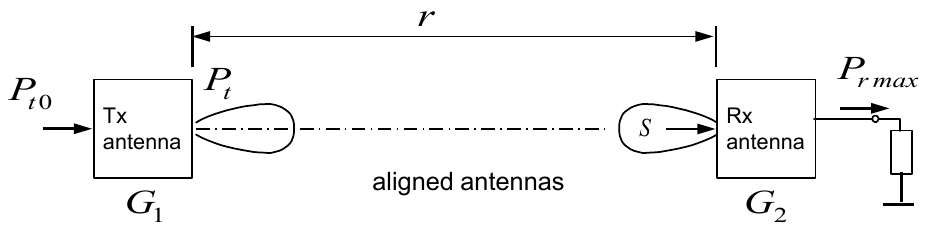
\includegraphics[width=.3\paperheight]{content/aawp/pictures/friis_transmission.png}
    \item \textbf{Friis Transmission Formula} for a radio link under far-field conditions:
        \begin{align}
            &\dfrac{P_{0,\text{RX}}}{P_{\text{A,TX}}} = G_{\text{TX}} G_{\text{RX}} \left(\dfrac{\lambda_0}{4\pi r} \right)^2,\label{eq:friis}\\
            &r: \text{distance between antennas},\nonumber\\
            &\lambda_0: \text{transmission wavelength},\nonumber\\
            &G_{\text{TX}}: \text{transmission antenna gain},\nonumber\\
            &G_{\text{RX}}: \text{receiving antenna gain}\nonumber
        \end{align}
    \item Radio Link Attenuation (\textit{Pathloss of free space}):\\
        \(\dfrac{a_0}{\si{dB}} = 10 \log_{10}^2\left(\dfrac{4 \pi r}{\lambda_0}\right) =\
        22 + 20 \log_{10}\left(\dfrac{r}{\lambda_0}\right)\)
\end{itemize}

\noindent\fbox{%
    \parbox{8cm}{%
        \textbf{How to Calculate Radiation Resistance} $R_r$:
        \begin{enumerate}
            \item Determine the antenna's current $I_a$ or its voltage $U_a$.
                \begin{equation*}
                    P_t = \dfrac{1}{2} |I_a|^2 R_r = \dfrac{1}{2} \dfrac{|U_a|^2}{R_r}
                \end{equation*}
            \item Equate the following with the above equation and solve for $R_r$:
                \begin{equation*}
                    P_t = \iint\limits_A \vec{S}(\vec{r}) \,\mathrm{d}\vec{A} = \iint\limits_A \dfrac{|E_{\mathrm{max}}|^2}{2 Z_F} |C(\vartheta,\varphi)|^2 \,\mathrm{d}\vec{A}
                \end{equation*}
        \end{enumerate}
    }}

		%%
		%\section{Gain Measurement}
Antenna gain measurements often make use of the Friis equation \eqref{eq:friis}.

\subsection{Two identical unknown antennas}

Absolute gain measure with two identical antennas.
Their characteristics don't have to be known, however they must be \textbf{as close to identical as possible}.
\begin{align}
  &G_{\text{TX}} = G_{\text{RX}} = G\nonumber\\
  \EqImplies{eq:friis} &G^{2}(\vartheta, \varphi) = \dfrac{P_{0,\text{RX}}}{P_{\text{A,TX}}} {\left(\dfrac{4\pi R}{\lambda}\right)}^{2}
\end{align}

\subsection{Three unknown antennas}
Abs.\ gain measure for three unknown antennas.
The procedure is as follows:
\begin{enumerate}
  \item Measure the antennas pairwise for transmitted power to use in Friis' equation.
  \item Solve the 3 resulting equations for the respective antenna gains.
\end{enumerate}

\begin{align*}
  &G_{{i,\text{dB}}} + G_{{j,\text{dB}}} = 20 \log_{10}\left(\dfrac{4\pi R}{\lambda}\right) + 10\,\log_{10}\left(\dfrac{P_{\text{RX},i}}{P_{\text{TX},j}}\right)\\
  &(i,j) = \{(1,2), (1,3), (2,3)\}
\end{align*}

\subsection{Gain Comparison}
Use a standard gain horn fo gain comparison to figure out the gain.
They're accurately reproducable, robust, ship with their gain curve and they have a low return loss.

\subsection{Direct Gain Measurement}
The idea is to measure an unknown AUT with a known probe, e.g.\ a standard gain horn.

\begin{equation*}
  G_{\text{AUT,dB}} = 20\log_{10}\left(\dfrac{4\pi R}{\lambda}\right) + 10\log_{10}\left(\dfrac{P_{\text{RX}}}{P_{\text{TX}}}\right) - G_{\text{probe,dB}}
\end{equation*}

\subsection{Measurement of Directivity and Efficiency}
Measure the relative intensity $U(\vartheta, \varphi)$ for all AUT orientations $(\vartheta, \varphi)$ in order to compute the directivity $D(\vartheta, \varphi)$:
\begin{equation}
  D(\vartheta, \varphi) = 4\pi \dfrac{U(\vartheta,\varphi)}{\oiint\limits_{\Omega}U(\vartheta, \varphi) \sin\vartheta\,\mathrm{d}\vartheta\mathrm{d}\varphi}.
\end{equation}

Then, measure the efficiency seperately, e.g.\ with a \textbf{Wheeler cap} or a \textbf{reverberation chamber} to get the gain:
\begin{equation*}
  G(\vartheta, \varphi) = \eta_{a} D(\vartheta, \varphi).
\end{equation*}

\subsection{Efficiency Measurement with a Wheeler Cap}
The idea is to make two antenna impedance measurements: one in free space and one with a Wheeler cap.

Und the assumption that the losses are mostly from internal antenna losses:
\begin{equation}
  \eta_{\text{AUT}} = \dfrac{P_{\text{free}} - P_{\text{cap}}}{P_{\text{free}}} = \dfrac{R_{\text{free}} - R_{\text{cap}}}{R_{\text{free}}}
\end{equation}

The radius of the cap is typically small, around $\lambda / (2\pi)$, roughly at the boundary between reactive and radiating near field.

		%\subsection{Reverberation Chamber}
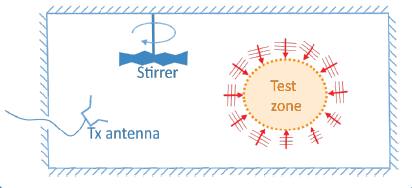
\includegraphics[width=8cm]{content/at_meas/pictures/reverberation_chamber}

A test chamber, contain ig a highly unsymmetric stirrer, designed to generate a \textbf{stochastical field distribution} in the test zone.

Ideally, it should have:
\begin{itemize}
  \item Electrically large cavity resonator with high $Q$ factor,
  \item High field strength for moderate input power,
  \item At least 60 resonant mode (IEEE 149--2022).
\end{itemize}

\subsection{Test Zone}
The ideal test zone field is:
\begin{itemize}
  \item isotropic (no preferred incident angle),
  \item homogenous (same magnitude everywhere),
  \item and unpolarized.
\end{itemize}

It can be described by a plane wave expansion:
\begin{equation}
  \bs{E}(\bs{r}) \oiint\limits_{\Omega} \bs{F}(\hat{\bs{k}}) \, e^{-j\bs{k}\cdot\bs{r}}\, \mathrm{d}^{2}\hat{\bs{k}}.
\end{equation}

		%\section{Radar Cross Section}

\begin{definition}{Radar Cross Section}
    Effective area which intercepts the transmitted radar and then scatters that power isotropically back to the radar receiver.
\end{definition}

\subsection{Scattering described by Dyadics}

Scattering object eclosed by arbitrary Huygens suface $\mathcal{S}$:
\begin{itemize}
        \item Incident fields uniquely determined by tangential fields $\bs{n}\times\bs{E}_{\mathrm{inc}}$ (and $\bs{n}\times\bs{H}_{\mathrm{inc}}$) on $\mathcal{S}$
        \item Scattered fields determined by equivalent surface currents $\bs{J}_{\mathrm{sca}}$, $\bs{M}_{\mathrm{sca}}$
        \item $\bs{J}_{\mathrm{sca}}$, $\bs{M}_{\mathrm{sca}}$ = linear function of $\bs{n}\times\bs{E}_{\mathrm{inc}}$, $\bs{n}\times\bs{H}_{\mathrm{inc}}$
\end{itemize}

General linear function by integral involving scattering dyadics $\DyadicS{E}{J}$, $\DyadicS{H}{J}$, $\DyadicS{E}{M}$, $\DyadicS{H}{M}$

\begin{align}
  \bs{J}_{\mathrm{sca}}(\bs{r}) = \oiint_{\mathcal{S}} \Big[ &\DyadicS{E}{J}\GreenRs \cdot \bs{E}(\bs{r}')\nonumber\\
  &+ \DyadicS{H}{J}\GreenRs\cdot\bs{H}(\bs{r}') \Big]\,\mathrm{d}a'
\end{align}

\begin{align}
  \bs{M}_{\mathrm{sca}}(\bs{r}) = \oiint_{\mathcal{S}} \Big[ &\DyadicS{E}{M}\GreenRs \cdot \bs{E}(\bs{r}')\nonumber\\
  &+ \DyadicS{H}{M}\GreenRs\cdot\bs{H}(\bs{r}') \Big]\,\mathrm{d}a'
\end{align}

\paragraph{Redundancy} Incident fields are completely determined by tangential electric or magnetic fields alone (except resonant edge cases) $\implies$ we can discard, e.g.\, $\DyadicS{H}{J}$ and $\DyadicS{H}{M}$.

Furthermore, scattered fields can be represented by electric or magnetic currents alone, therefore e.g.\ only $\DyadicS{E}{J}$ is required.

\subsection{Polarization Scattering Matrix}
Models an incident plane wave from $\vartheta'$, $\varphi'$-direction and a scattered far-field $\bs{F}^{\mathrm{sca}}(\vartheta, \varphi) = \lim\limits_{r\to\infty} \frac{r}{e^{-jkr}} \, \bs{E}^{\mathrm{sca}}(r, \vartheta, \varphi)$.

Decomposed into co- and cross-polar components:

		%\section{Polarization}

\begin{definition}{Polarization Basis}
  Well-defined (complex) unit vector distribution tangential to far-field sphere (unit normal $\bs{n}$).
\end{definition}

\begin{equation*}
  \bs{e}_{\text{cr}}(\vartheta,\varphi) = \bs{n}(\vartheta,\varphi) \times \bs{e}_{\text{co}}^{*}(\vartheta, \varphi)
\end{equation*}

$\bs{C}(\vartheta,\varphi)$ can be decomposed into components:

\begin{align*}
  &\bs{C}(\vartheta,\varphi) = C_{\text{co}}\bs{e}_{\text{co}} + C_{\text{cr}}\bs{e}_{\text{cr}},\\
  &C_{\text{co/cr}} = \bs{C}(\vartheta,\varphi) \cdot \bs{e}_{\text{co/cr}}^{*}(\vartheta,\varphi).
\end{align*}

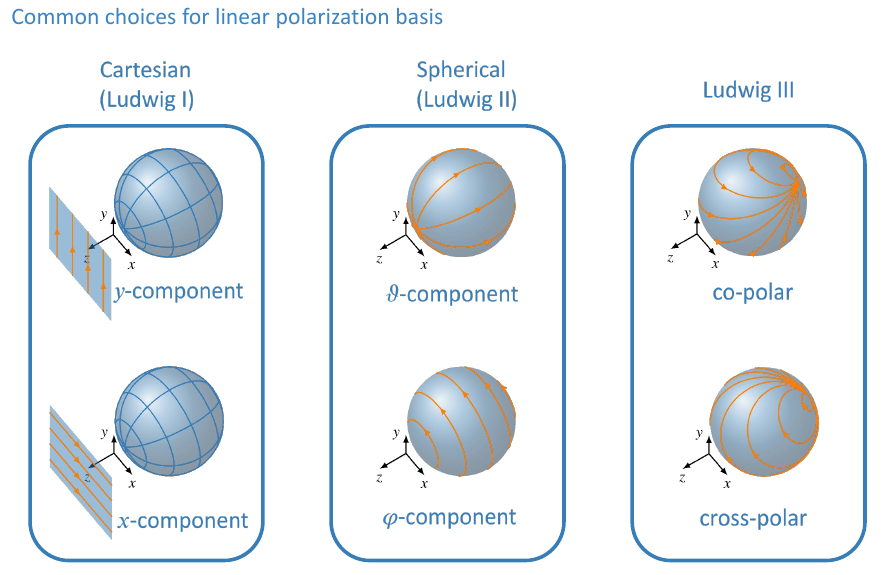
\includegraphics[angle=90, height=7cm]{content/at_meas/pictures/linear_polarization_bases}

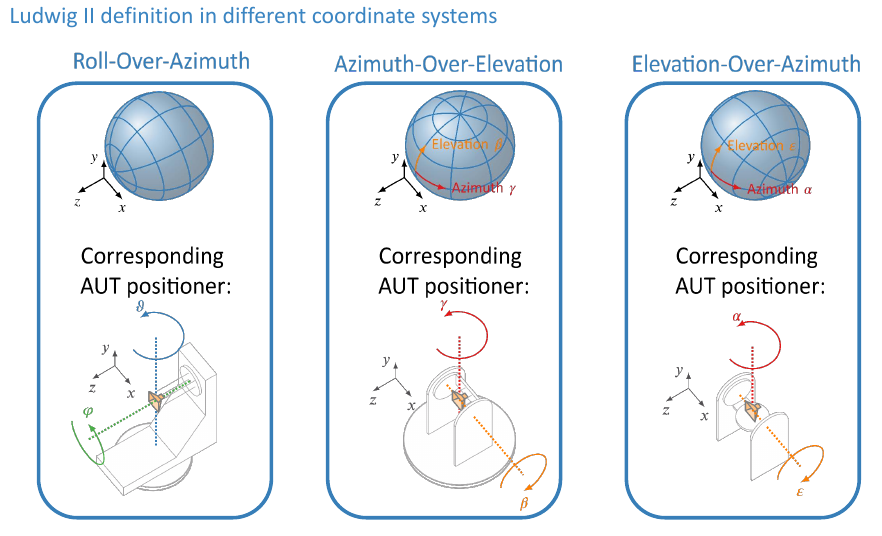
\includegraphics[angle=90, height=7cm]{content/at_meas/pictures/ludwig_II}

\subsection{Conversion between Linear Polarization Bases}


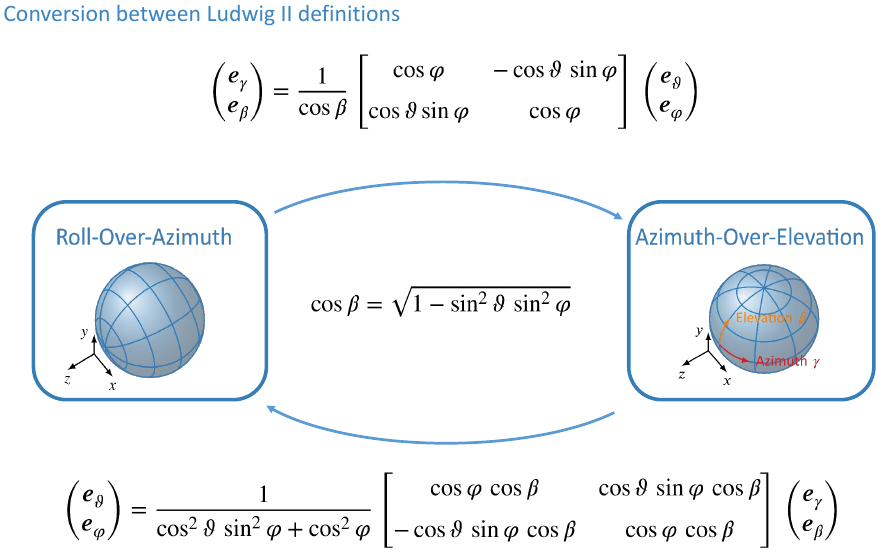
\includegraphics[width=8.5cm]{content/at_meas/pictures/ludwig_II_conversion1}
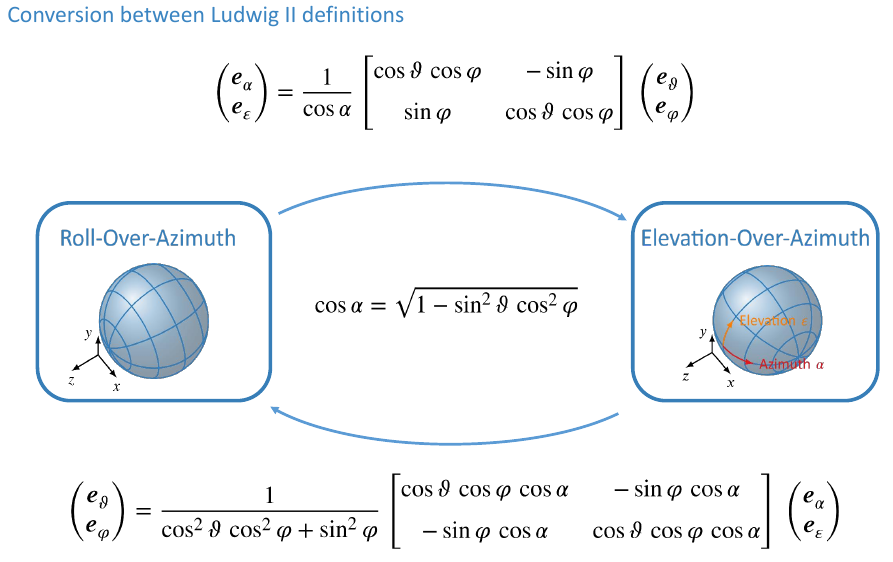
\includegraphics[width=8.5cm]{content/at_meas/pictures/ludwig_II_conversion2}

Conversion between Ludwig II and Ludwig III basis:

\begin{equation*}
  \begin{pmatrix}
    \bs{e}_{\text{co,3L}}\\
    \bs{e}_{\text{cr,3L}}
  \end{pmatrix}
  =
  \begin{bmatrix}
    \cos(\varphi - \varphi_{0}) & - \sin(\varphi - \varphi_{0})\\
    \sin(\varphi - \varphi_{0}) & \cos(\varphi - \varphi_{0})
  \end{bmatrix}
  \begin{pmatrix}
    \bs{e}_{\vartheta}\\
    \bs{e}_{\varphi}
  \end{pmatrix}
\end{equation*}

\begin{equation*}
  \begin{pmatrix}
    \bs{e}_{\vartheta}\\
    \bs{e}_{\varphi}
  \end{pmatrix}
  =
  \begin{bmatrix}
    \cos(\varphi - \varphi_{0}) & \sin(\varphi - \varphi_{0})\\
    - \sin(\varphi - \varphi_{0}) & \cos(\varphi - \varphi_{0})
  \end{bmatrix}
  \begin{pmatrix}
    \bs{e}_{\text{co,3L}}\\
    \bs{e}_{\text{cr,3L}}
  \end{pmatrix}
\end{equation*}

$\varphi_{0} = 0 \implies \bs{e}_{\text{co,3L}} = \bs{e}_{x}$ in main radiation direction ($\bs{e}_{z}$).

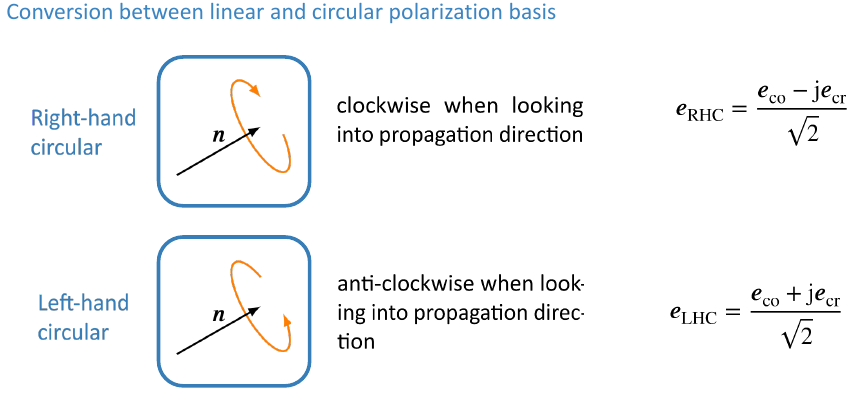
\includegraphics[width=7.5cm]{content/at_meas/pictures/linear_and_circular_polarization_conversion}

\subsection{Elliptical Polarization}

The most general case.\\
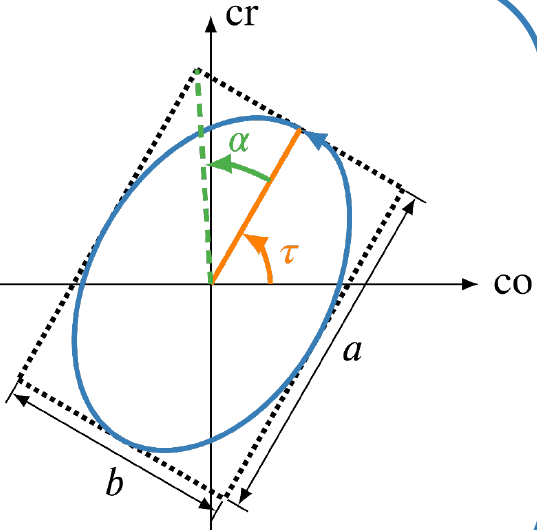
\includegraphics[width=3cm]{content/at_meas/pictures/elliptical_polarization}\\
\begin{itemize}
    \item Tilt angle
    \begin{equation*}
      \tau = \dfrac{\angle(C_{\text{LHC}}) - \angle(C_{\text{RHC}})}{2} = -\dfrac{\delta_{c}}{2}
    \end{equation*}
   \item Axial Ratio
   \begin{equation*}
     r = \dfrac{a}{b} = \dfrac{1}{\tan \alpha} = \dfrac{|C_{\text{RHC}}| + |C_{\text{LHC}}|}{|C_{\text{RHC}}| - |C_{\text{LHC}}|} = \dfrac{|\rho_{C}| + 1}{|\rho_{C}| - 1}
   \end{equation*}
  $r = \infty$ $\implies$ linear\\
  $r = 1$ $\implies$ circular\\
  $1 < r < \infty$ $\implies$ elliptical\\
  $\rho_{C} = \dfrac{C_{\text{RHC}}}{C_{\text{LHC}}}, \quad \delta_{C} = \angle(\rho_{C})$
\end{itemize}


\subsection{Poincaré Sphere}

\begin{center}
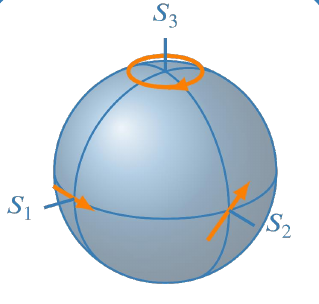
\includegraphics[width=5cm]{content/at_meas/pictures/poincare_sphere}
\end{center}

Stokes Parameters:

\begin{align*}
  &S_{0} = {|E_{co}|}^{2} + {|E_{cr}|}^{2} = {|E_{\text{LHC}}|}^{2} + {|E_{\text{RHC}}|}^{2}\\
  &S_{1} = {|E_{co}|}^{2} - {|E_{cr}|}^{2}\\
  &S_{2} = {|E_{45°}|}^{2} - {|E_{135°}|}^{2}\\
  &S_{3} = {|E_{\text{LHC}}|}^{2} - {|E_{\text{RHC}}|}^{2}\\
\end{align*}

\begin{align*}
  p = \dfrac{\sqrt{S_{1}^{2} + S_{2}^{2} + S_{3}^{2}}}{S_{0}}: \quad \text{degree of polarization}
\end{align*}

		%\input{content/at_meas/antenna_test_ranges}
		%\section{Measurement Hardware}
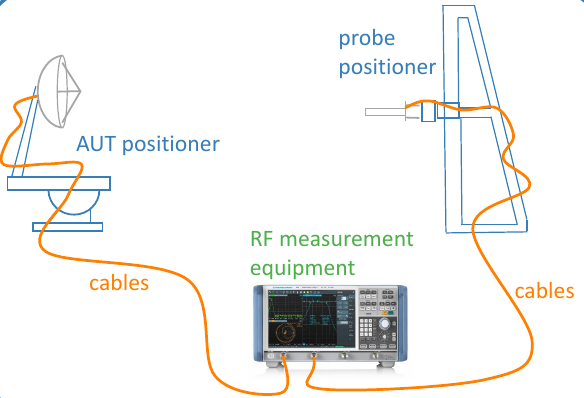
\includegraphics[width=7cm]{content/at_meas/pictures/measurement_hardware}
\begin{itemize}
  \item Network Analyzer (Magn.+Phase, one freq.\ at a time)
  \item Spectrum Analyzer (Broadband, low temp.\ resolution)
  \item Oscilloscope (Hight temporal resolution, up to \SI{10}{GHz})
\end{itemize}

		%\input{content/at_meas/measurement_errors}
		%\input{content/at_meas/nf_measurements}
		%\input{content/at_meas/echo_suppression}
	\end{multicols*}
\end{document}
